\thispagestyle{cackithitoannone}
\pagestyle{cackithitoan}
\everymath{\color{cackithi}}
\graphicspath{{../cackithi/pic/}}
\blfootnote{\color{cackithi}$^1$Khoa Toán Đại học Osnabrueck, CHLB Đức.}
\begingroup
\AddToShipoutPicture*{\put(0,616){
\includegraphics[width=19.3cm]{../bannercackithi}}}
\AddToShipoutPicture*{\put(82,527){
\includegraphics[scale=1]{../tieude2.pdf}}}
\centering
\endgroup
\vspace*{182pt}

\begin{multicols}{2}
	Kỳ thi toán học liên bang của Đức (Bundeswettbewerb Mathematik) được tổ chức lần đầu tiên vào năm $1970$ tại Cộng hòa liên bang Đức (Tây Đức) dưới sự bảo trợ của Hiệp hội tài trợ cho khoa học Đức, Bộ Giáo dục và Khoa học liên bang cùng các doanh nghiệp. Sau khi nước Đức thống nhất, kỳ thi đã được mở rộng thành kỳ thi quốc gia. 
	\begin{figure}[H]
		\vspace*{-5pt}
		\centering
		\captionsetup{labelformat= empty, justification=centering}
		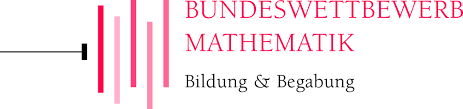
\includegraphics[width= 1\linewidth]{2}
		\caption{\small\textit{\color{cackithi}Logo của Kỳ thi toán học liên bang Đức.}}
		\vspace*{-10pt}
	\end{figure}
	Kỳ thi toán học liên bang kéo dài khoảng $14$ tháng với ba vòng thi, trong đó hai vòng thi đầu là bài tập về nhà và vòng thi cuối là thảo luận toán học. Ở mỗi vòng bài tập về nhà các thí sinh có nhiều tháng để suy nghĩ về các câu hỏi trước khi đưa ra lời giải. Ở vòng thi cuối, thí sinh sẽ có một giờ đồng hồ để thảo luận toán học với các nhà toán học. Mô hình này bị ảnh hưởng bởi một thực tế là những vấn đề của toán học thường cần nhiều tháng đến nhiều năm để có thể có một bước tiến chứ không phải vài giờ đồng hồ. Ngoài ra, để có thể thành công trong toán học, bên cạnh kỹ năng giải toán thì kỹ năng trao đổi và truyền đạt cũng thực sự cần thiết. 
	\vskip 0.1cm
	Nội dung của kỳ thi toán học liên bang phù hợp với học sinh từ lớp $9$ đến lớp $13$. Tuy vậy, tất cả học sinh ở Đức với mọi lứa tuổi mà có sự đam mê và kiên trì đều được khuyến khích tham gia. Những thí sinh đạt giải ở vòng một sẽ được mời tham gia vòng hai. Những thí sinh giành giải nhất ở vòng hai sẽ được mời tham gia vòng thảo luận toán học. Phần thưởng cho những người chiến thắng ở vòng cuối sẽ là những suất học bổng có giá trị để họ tiếp tục theo đuổi con đường học tập và nghiên cứu sau này. Ngoài ra, những thí sinh đạt giải cao ngay ở vòng hai sẽ được mời tham dự kỳ thi tuyển chọn học sinh đại diện cho nước Đức tham gia kỳ thi Olympic toán học quốc tế.
	\vskip 0.1cm
	Hiện tại, kỳ thi toán học liên bang năm $2023$ đang ở vòng thứ hai. Vòng thi này sẽ kết thúc vào ngày $01.09.2023$. Pi mời các độc giả cùng thử sức với đề thi năm nay nhé!
	\vskip 0.1cm
	\textbf{\color{cackithi}Vòng $\pmb{1.}$}
	\vskip 0.1cm
	\textbf{\color{cackithi}Câu $\pmb{1}$}: Ba bạn Tick, Trick và Track có $20$, $23$ và $25$ vé để đi vòng quay ngựa gỗ tại hội chợ hàng năm. Họ thống nhất rằng sẽ chỉ đi vòng quay nếu cả ba cùng đi và mỗi người nộp một vé của mình. Ngoài ra, trước mỗi lần đi, nếu muốn, họ có thể chia lại vé cho nhau bao nhiêu lần tùy thích theo quy tắc sau: Người nào có số vé chẵn thì có thể chia một nửa số vé của mình cho một trong hai người còn lại. Hỏi có thể xảy ra rằng sau một lần đi nào đó:
	\vskip 0.1cm
	$\bullet$ Đúng một người hết vé.
	\vskip 0.1cm
	$\bullet$ Đúng hai người hết vé.
	\vskip 0.1cm
	$\bullet$ Cả ba cùng hết vé. 
	\vskip 0.1cm
	\textbf{\color{cackithi}Câu $\pmb{2}$}: Tìm tất cả các bộ ba số nguyên $(x,y,z)$ thỏa mãn phương trình 
	\begin{align*}
		x^2 + y^2 + z^2 -xy-yz-zx = 3.
	\end{align*}
	\textbf{\color{cackithi}Câu $\pmb{3}$}: Cho hai hình bình hành $ABCD$ và $AECF$ có chung đường chéo $AC$, trong đó $E$ và $F$ nằm bên trong $ABCD$. Chứng minh rằng đường tròn ngoại tiếp của các tam giác $AEB$, $BFC$, $CED$ và $DFA$ giao nhau tại một điểm. 
	\vskip 0.1cm
	\textbf{\color{cackithi}Câu $\pmb{4}$}:  Cho số thực $\alpha$ với biểu diễn thập phân $\alpha = 0,a_1 a_2 a_3 \ldots$ trong đó mỗi chữ số $a_i$ là một số nguyên tố. Các chữ số sau dấu phẩy được sắp xếp dọc theo đường được tạo ra bởi các mũi tên như trong hình bên, được tưởng tượng là tiếp tục vô tận về bên phải và xuống dưới.
	\begin{figure}[H]
		\vspace*{-5pt}
		\centering
		\captionsetup{labelformat= empty, justification=centering}
		\begin{tikzpicture}[cackithi, scale=0.8]
			\draw (0,4) node {$a_1$};
			\draw (1.5,4) node {$a_2$};
			\draw (1.5,2.5) node {$a_3$};
			\draw (0,2.5) node {$a_4$};
			\draw (0,1) node {$a_5$};
			\draw (1.5,1) node {$a_6$};
			\draw (3,1) node {$a_7$};
			\draw (3,2.5) node {$a_8$};
			\draw (3,4) node {$a_9$};
			\draw (4.5,4) node {$a_{10}$};
			\draw (4.5,2.5) node {$a_{11}$};
			\draw (4.5,1) node {$a_{12}$};
			\draw (4.5,-0.5) node {$a_{13}$};
			\draw (3,-0.5) node {$a_{14}$};
			\draw (1.5,-0.5) node {$a_{15}$};
			\draw (0,-0.5) node {$a_{16}$};
			\draw (0,-2) node {$a_{17}$};
			\draw (1.5,-2) node {$a_{18}$};
			\draw (3,-2) node {$a_{19}$};
			\draw (4.5,-2) node {$a_{20}$};
			\draw (6,-2) node {$a_{21}$};
			\draw (6,-0.5) node {$a_{22}$};
			\draw (6,1) node {$a_{23}$};
			\draw (6,2.5) node {$a_{24}$};
			\draw (6,4) node {$a_{25}$};
			\draw (7.5,4) node {$a_{26}$};
			\draw (7.5,2.5) node {$a_{27}$};
			\draw (7.5,1) node {$a_{28}$};
			\draw [-stealth] (.5,4) -- (1,4);
			\draw [-stealth] (1.5,3.5) -- (1.5,3);
			\draw [-stealth] (1,2.5) -- (0.5,2.5);
			\draw [-stealth] (0,2) -- (0,1.5);
			\draw [-stealth] (0.5,1) -- (1,1);
			\draw [-stealth] (2,1) -- (2.5,1);
			\draw [-stealth] (3,1.5) -- (3,2);
			\draw [-stealth] (3,3) -- (3,3.5);
			\draw [-stealth] (3.5,4) -- (4,4);
			\draw [-stealth] (4.5,3.5) -- (4.5,3);
			\draw [-stealth] (4.5,2) -- (4.5,1.5);
			\draw [-stealth] (4.5,0.5) -- (4.5,0);
			\draw [-stealth] (4,-0.5) -- (3.5,-0.5);
			\draw [-stealth] (2.5,-0.5) -- (2,-0.5);
			\draw [-stealth] (1,-0.5) -- (0.5,-0.5);
			\draw [-stealth] (0,-1) -- (0,-1.5);
			\draw [-stealth] (0.5,-2) -- (1,-2);
			\draw [-stealth] (2,-2) -- (2.5,-2);
			\draw [-stealth] (3.5,-2) -- (4,-2);
			\draw [-stealth] (5,-2) -- (5.5,-2);
			\draw [-stealth] (6,-1.5) -- (6,-1);
			\draw [-stealth] (6,0) -- (6,0.5);
			\draw [-stealth] (6,1.5) -- (6,2);
			\draw [-stealth] (6,3) -- (6,3.5);
			\draw [-stealth] (6.5,4) -- (7,4);
			\draw [-stealth] (7.5,3.5) -- (7.5,3);
			\draw [-stealth] (7.5,2) -- (7.5,1.5);
			\draw (7.5, 0.33) node {$\vdots$};
		\end{tikzpicture}
		\vspace*{-5pt}
	\end{figure}
	Với mỗi $m \ge 1$, biểu diễn thập phân của số thực $z_m$ được cho bằng cách viết chữ số $0$ trước dấu phẩy và sau dấu phẩy là các chữ số của dòng thứ $m$ (tính từ trên xuống) theo thứ tự từ trái sang phải. Tương tự, với mọi $n \ge 1$, số thực $s_n$ được thiết lập với các chữ số của cột thứ $n$ (tính từ bên trái sang) theo thứ tự từ trên xuống dưới. Chẳng hạn $z_3 = 0, a_5a_6a_7a_{12}a_{23}a_{28}\ldots$ và $s_2 = 0,a_2a_3a_6a_{15}a_{18}a_{35}\ldots$. Chứng minh rằng:
	\vskip 0.1cm
	$(a)$ Nếu $\alpha$ là số hữu tỷ, thì tất cả các số $z_m$ và $s_n$ đều hữu tỷ.
	\vskip 0.1cm
	$(b)$ Điều ngược lại của khẳng định $(a)$ là sai.
	\vskip 0.1cm
	\textbf{\color{cackithi}Vòng $\pmb{2.}$}
	\vskip 0.1cm
	\textbf{\color{cackithi}Câu $\pmb{1}$}: Tìm ước chung lớn nhất của tất cả các số có dạng $p^6 - 7p^2 +6$ với $p$ chạy trên tập tất cả các số nguyên tố và $p \ge 11$.
	\vskip 0.1cm
	\textbf{\color{cackithi}Câu $\pmb{2}$}: Trên một hòn đảo địa hình đồi núi có $2023$ điểm quan sát. Từ mỗi điểm quan sát có thể nhìn thấy ít nhất $42$ điểm quan sát khác. Với hai điểm quan sát bất kỳ $X$ và $Y$, luôn tồn tại một số nguyên dương $n$ và các điểm quan sát $A_1,  A_2, \ldots, A_{n+1}$ sao cho $A_1 = X$, $A_{n+1} = Y$ và mỗi cặp điểm liền kề $A_i$ với $A_{i+1}$ có thể quan sát được lẫn nhau với $i = 1, 2, \ldots, n$. Số $n$ nhỏ nhất như vậy được gọi là khoảng cách quan sát (Sichtabstand). 
	\vskip 0.1cm
	Xác định khoảng cách quan sát lớn nhất có thể có giữa hai cặp điểm quan sát thỏa mãn những điều kiện ở trên.
	\vskip 0.1cm
	\textbf{\color{cackithi}Câu $\pmb{3}$}: Cho tam giác $AB$C với tâm đường tròn nội tiếp $I$. Gọi trung điểm của các cạnh $AC$ và $BC$ lần lượt là $M_b$ và $M_a$. Gọi giao điểm của đường thẳng $M_bI$ với đường thẳng $BC$ là $B'$ và giao điểm của đường thẳng $M_aI$ với đường thẳng $AC$ là $A'$. Biết rằng hai tam giác $ABC$ và $A'B'C$ có cùng diện tích. 
	\vskip 0.1cm
	Tìm giá trị lớn nhất có thể của góc $ACB$.
	\vskip 0.1cm
	\textbf{\color{cackithi}Câu $\pmb{4}$}: Cho một đa diện đều $2n$ cạnh. Từ các đoạn thẳng nối các đỉnh của đa diện (cạnh biên hoặc đường chéo) ta tô $n$ cạnh màu đỏ sao cho:
	\vskip 0.1cm
	$1.$ Các điểm cuối của các cạnh màu đỏ chính là $2n$ đỉnh của đa diện.
	\vskip 0.1cm
	$2.$  Không có $2$ cạnh màu đỏ nào có độ dài bằng nhau.
	\vskip 0.1cm
	Tìm tất cả các số tự nhiên $n \ge 2$ thỏa mãn yêu cầu đã cho.
\end{multicols}
\newpage
\begingroup
\AddToShipoutPicture*{\put(150,695){
\includegraphics[scale=1]{../tieude1.pdf}}}
\centering
\endgroup
\vspace*{10pt}

\begin{multicols}{2}
	Trong phần đầu chuyên mục, chúng tôi sẽ trình bày với các bạn lời giải của các bài toán trong kỳ thi Olympic toán học trẻ của Thổ Nhĩ Kỳ, đăng trong số báo $5/2023$. 
	\begin{figure}[H]
		\vspace*{-5pt}
		\centering
		\captionsetup{labelformat= empty, justification=centering}
		
\includegraphics[width= 1\linewidth]{gocolympic}
		%		\caption{\small\textit{\color{}}}
		\vspace*{-10pt}
	\end{figure}
	{\bf\color{cackithi} OC$\pmb{40.}$} Cho $x, y, z$ là các số thực dương với $x\le 1.$ Chứng minh rằng
	\begin{align*}
		xy+y+2z \geq 4 \sqrt{xyz}.
	\end{align*}
	\textit{Lời giải.} Trong bài này có thể dùng giả thiết $x\le 1$ theo các cách khác nhau dẫn đến những lời giải khác nhau.
	\vskip 0.1cm
	\textit{Lời giải} $1$: từ $x\le 1$ ta có $z \ge zx.$ Kết hợp với bất đẳng thức Cauchy, ta thu được điều cần chứng minh
	\begin{align*}
		xy+y+2z &\ge  xy \!+\!y \!+\! z \!+\! zx = (x\!+\!1)(y\!+\!z) \\
		&\ge 2\sqrt{x}2\sqrt{yz}= 4 \sqrt{xyz}.
	\end{align*}
	\textit{Lời giải} $2$: theo bất đẳng thức Cauchy, ta có $ xy+y+2z=(x+1)y+ 2z \ge 2\sqrt{(x+1)y2z}.$ Từ giả thiết $x\le 1$ ta có $x+1\ge 2x,$ như vậy ta có điều cần chứng minh
	\begin{align*}
		xy+y+2z &\ge 2\sqrt{(x+1)y2z}\\
		&\ge 2\sqrt{2xy2z}= 4\sqrt{xyz}.
	\end{align*} 
	
	{\bf\color{cackithi} OC$\pmb{41.}$} Trong một trường có $101$ học sinh, mỗi học sinh có ít nhất một người bạn thân trong số các học sinh khác trong trường. Chứng minh rằng với mọi số nguyên $n, 1<n<101,$ ta có thể chọn một nhóm $n$ học sinh trong trường này sao cho mỗi học sinh được chọn có ít nhất một bạn thân trong số các học sinh khác được chọn. (Biết rằng nếu  $A$ là bạn thân của $B$ thì $B$ cũng là bạn thân của $A$).
	\vskip 0.1cm
	\textit{Lời giải.}
	Với $n=2,$ kết luận đúng vì ta chỉ cần chọn ra $1$ học sinh cùng với $1$ bạn thân của người đó.
	\vskip 0.1cm
	Nếu ta gọi $d_i$ là số bạn thân mà học sinh thứ $i$ có thì tổng $s=\sum_{i=1}^{101} d_i$ phải là số chẵn vì mỗi cặp bạn thân được tính $2$ lần trong tổng. Độc giả nào biết về lý thuyết đồ thị sẽ nhận ra ngay đây là một kết quả quen thuộc, thường được gọi là Bổ đề bắt tay. Như vậy không thể xảy ra trường hợp mỗi học sinh chỉ có đúng $1$ bạn thân vì khi đó $s=101,$ là số lẻ. Do đó, ta có thể chọn ra một bạn $A$ có ít nhất $2$ bạn thân. Nhóm gồm bạn $A$ và $2$ bạn thân của $A$ thỏa mãn điều kiện đầu bài, tức là kết luận đúng với $n=3$.
	\vskip 0.1cm
	Ta sẽ chứng minh rằng từ nhóm $G$ bất kỳ gồm $n<100$ học sinh thỏa mãn đầu bài, ta luôn có thể thêm vào $2$ học sinh nữa để nhận được nhóm cũng thỏa mãn đầu bài. Thật vậy, xét hai học sinh $A, B$ không thuộc $G.$ Nếu $A$ hoặc $B$ có một bạn thân không nằm trong $G$ thì ta có $1$ cặp bạn thân không thuộc $G.$ Bổ sung cặp bạn thân này vào $G,$ ta được nhóm mới vẫn thỏa mãn đầu bài. Trường hợp còn lại, cả $A$ và $B$ đều phải có bạn thân trong $G,$ lúc này nhóm $G\cup \{A, B\}$ hiển nhiên thỏa mãn đầu bài.
	\vskip 0.1cm
	Như vậy, xuất phát với nhóm gồm $2$ hoặc $3$ học sinh thỏa mãn đầu bài ta có thể xây dựng được nhóm $n$ học sinh thỏa mãn đầu bài với mọi $1<n<101.$    
	\vskip 0.1cm
	{\bf\color{cackithi} OC$\pmb{42.}$} Cho $m, n, a, k$ là các số nguyên dương và $k>1$ sao cho đẳng thức sau thỏa mãn
	\begin{align*}
		5^m+63n+49=a^k.
	\end{align*}
	Tìm giá trị nhỏ nhất của $k$.
	\vskip 0.1cm
	\textit{Lời giải.} Ta sẽ chứng minh trường hợp $k=2, 3, 4$ không xảy ra.
	\vskip 0.1cm
	Giả sử $k=2,$ xét đẳng thức $5^m+63n+49=a^k$ modulo $7$ ta có 
	\begin{align*}
		5^m \equiv a^2 \equiv 0,1,2,4 \pmod{7}.
	\end{align*}
	Do $5^6\equiv 1 \pmod{7},$  ta nhận được $m \equiv 0,2,4 \pmod{6}.$ 
	\vskip 0.1cm
	Như vậy $m$ là số chẵn. Tiếp tục xét modulo $3$, ta có
	\begin{align*}
		5^m+63n+49 \equiv (-1)^{m}+1  \equiv 2 \pmod{3}.
	\end{align*}
	Tuy nhiên điều này dẫn đến $a^2\equiv 2 \pmod{3},$ mâu thuẫn.  
	\vskip 0.1cm
	Giả sử $k=3,$ xét modulo $7$, ta có
	\begin{align*}
		5^m \equiv a^3 \equiv 0,1,6 \pmod{7}.
	\end{align*}
	Từ đó suy ra ra $m \equiv 0,3 \pmod{6},$ tức là $m=3l.$
	\vskip 0.1cm
	Tiếp tục xét modulo $9$, ta có 
	\begin{align*}
		5^m+63n+49 &\equiv (5)^{3l}+4  \equiv (-1)^l +4\\
		&\equiv 3, 5 \pmod{9}.
	\end{align*}
	Tuy nhiên điều này dẫn đến mâu thuẫn vì $a^3\equiv 0, 1, 8 \pmod{9}.$
	\vskip 0.1cm
	Do trường hợp $k=2$ không xảy ra nên $k=4$ cũng không xảy ra vì ta có thể viết $5^m+63n+49=a^4=(a^2)^2.$
	\vskip 0.1cm
	Trường hợp $k=5,$ ta tìm được bộ $m=1, n=3, a=3$ thỏa mãn đẳng thức. Như vậy giá trị nhỏ nhất có thể của $k$ là $5$.
	\vskip 0.1cm
	Trong phần cuối của chuyên mục kỳ này, chúng tôi sẽ giới thiệu với bạn đọc ba bài toán trong Kỳ thi toán Durer lần thứ XVI được tổ chức tại Hungary. Đây là kỳ thi toán đồng đội mang tên Albrecht Durer, một nghệ sĩ, nhà tư tưởng nổi tiếng thời kỳ Phục hưng. Các bài toán sau phù hợp với trình độ học sinh lớp $7-9$.
	\vskip 0.1cm
	{\bf\color{cackithi} OC$\pmb{49.}$} Cho $ABC$ là tam giác cân. Cạnh đáy $BC$ dài $1$ cm, cạnh $AB$ và $AC$ dài $2$ cm. Gọi $F$ là trung điểm của $AB$ và $G$ là trung điểm của $AC.$ Gọi $(k)$ là đường tròn tiếp xúc với $AB$ và $AC$, tương ứng tại $F$ và $G$. Chứng minh rằng giao điểm của $CF$ và $BG$ thuộc đường tròn $(k).$
	\vskip 0.1cm
	{\bf\color{cackithi} OC$\pmb{50.}$} Khi Andris bước vào phòng, có các số $3$ và $24$ trên bảng. Trong một bước, nếu đã có các số (không nhất thiết phải khác nhau) $k$ và $n$ trên bảng, thì
	Andris có thể viết thêm số $kn + k + n$ lên bảng. 
	\vskip 0.1cm
	$(a)$ Liệu Andris có thể viết số  $9999999$ lên bảng sau một số bước?
	\vskip 0.1cm
	$(b)$ Cùng câu hỏi như phần $(a)$ cho số $99999999$?
	\vskip 0.1cm
	$(c)$ Cùng câu hỏi như phần $(a)$ cho số $48999999$?
	\vskip 0.1cm
	{\bf\color{cackithi} OC$\pmb{51.}$} Có một trò chơi với một bảng ô vuông cỡ $3 \times 3$. Trong mỗi bước, người chơi lần lượt điền một trong các số $1$, $2$ hoặc $3$ vào một ô trống sao cho không có hai số giống nhau trong cùng một hàng hoặc trong cùng một cột. Nếu tất cả $9$ ô của bảng đều được điền số, người chơi đầu tiên thắng nhưng nếu trước đó có một thời điểm không thể điền số được nữa thì người chơi thứ hai thắng.
	\vskip 0.1cm
	Hỏi có cách nào để luôn chiến thắng nếu bạn được phép tùy chọn đi trước hoặc đi sau?
\end{multicols}